% =============================================================================
% Section 7: Country Profiles
% =============================================================================
\section{Country Profiles}\label{sec:country-profiles}

This section presents radar-chart profiles for eight selected
countries, chosen to represent the full range of ISI composites
and diverse axis configurations.  Each radar chart displays the
country's score on each of the six axes, with the outer ring fixed
at~1.0.  We then examine geographic and structural correlates of the
composite ISI.

\subsection{Selection rationale}

The eight countries were selected to cover:
\begin{itemize}[leftmargin=2em]
  \item \textbf{Top of the ranking}: Malta (rank~1), Cyprus (rank~2).
  \item \textbf{Upper-middle}: Ireland (rank~3), Finland (rank~6).
  \item \textbf{Mid-range}: Netherlands (rank~15).
  \item \textbf{Lower ranks}: Germany (rank~22), Slovakia (rank~26),
    France (rank~27).
  \item \textbf{Diverse axis profiles}: Ireland (technology-peaked),
    Netherlands (defence-peaked), Finland (critical-inputs-peaked),
    Slovakia (zero-defence outlier).
\end{itemize}

\subsection{Malta (Rank 1, ISI = 0.5175)}

Malta records the highest composite score in the EU-27 and is the
only country classified as \emph{highly concentrated}.  Its profile
is dominated by defence (1.000) and logistics (1.000)---both at the
theoretical maximum.  The financial axis (0.140) and technology axis
(0.205) are comparatively moderate.  Malta's small-island economy
and NATO membership channel its defence imports through a single
dominant supplier, while its port infrastructure concentrates
logistics flows.

\begin{figure}[htbp]
\centering
\input{figures/F08_radar_MT}
\caption{ISI axis profile: Malta.  Composite ISI = 0.5175 (rank~1,
  highly concentrated).}
\label{fig:radar-MT}
\end{figure}

\subsection{Cyprus (Rank 2, ISI = 0.4682)}

Cyprus ranks second with a profile similar to Malta's: defence
(0.748) and logistics (0.941) dominate, but neither reaches the
boundary.  Critical inputs (0.424) is also elevated relative to
the EU-27 mean.  Like Malta, Cyprus's small size and island geography
concentrate its strategic dependencies.

\begin{figure}[htbp]
\centering
% F09_radar_CY: Radar chart for Cyprus (CY)
% Values: Fin=0.124, Ene=0.348, Tec=0.224, Def=0.748, Cri=0.424, Log=0.941
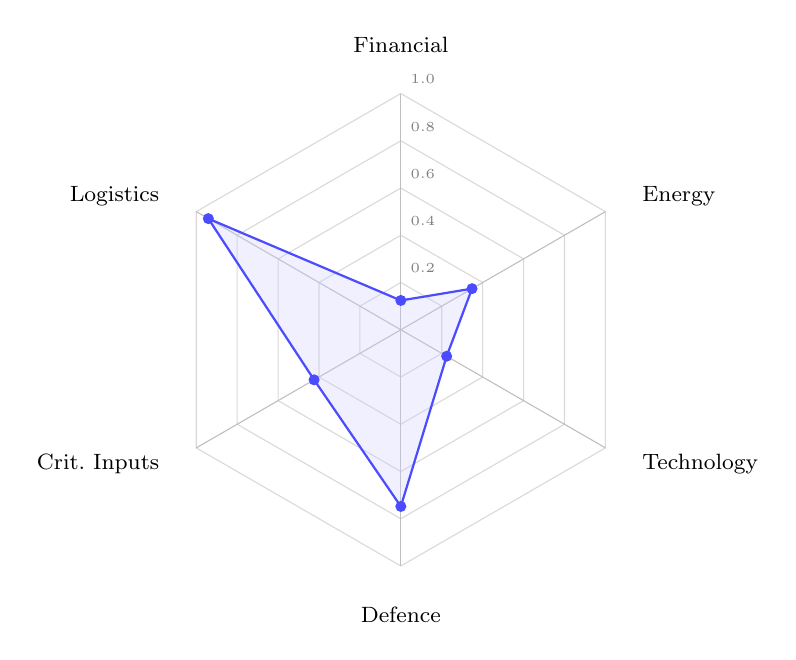
\begin{tikzpicture}[scale=1.0]
  % Grid rings
  \foreach \r in {0.2, 0.4, 0.6, 0.8, 1.0} {
    \draw[gray!30, thin]
      ( 90:\r*3cm) -- ( 30:\r*3cm) -- (330:\r*3cm) --
      (270:\r*3cm) -- (210:\r*3cm) -- (150:\r*3cm) -- cycle;
  }
  % Axis spokes
  \foreach \a in {90, 30, 330, 270, 210, 150} {
    \draw[gray!50, thin] (0,0) -- (\a:3cm);
  }
  % Axis labels
  \node[font=\footnotesize, above] at ( 90:3.4cm) {Financial};
  \node[font=\footnotesize, right] at ( 30:3.4cm) {Energy};
  \node[font=\footnotesize, right] at (330:3.4cm) {Technology};
  \node[font=\footnotesize, below] at (270:3.4cm) {Defence};
  \node[font=\footnotesize, left] at (210:3.4cm) {Crit.~Inputs};
  \node[font=\footnotesize, left] at (150:3.4cm) {Logistics};
  % Ring labels
  \foreach \r/\lab in {0.2/0.2, 0.4/0.4, 0.6/0.6, 0.8/0.8, 1.0/1.0} {
    \node[font=\tiny, gray, anchor=south west] at (90:\r*3cm) {\lab};
  }
  % Data polygon: CY
  \filldraw[blue!20, draw=blue!70, thick, fill opacity=0.3]
    ( 90:0.124*3cm) -- ( 30:0.348*3cm) -- (330:0.224*3cm) --
    (270:0.748*3cm) -- (210:0.424*3cm) -- (150:0.941*3cm) -- cycle;
  % Data points
  \fill[blue!70] ( 90:0.124*3cm) circle (2pt);
  \fill[blue!70] ( 30:0.348*3cm) circle (2pt);
  \fill[blue!70] (330:0.224*3cm) circle (2pt);
  \fill[blue!70] (270:0.748*3cm) circle (2pt);
  \fill[blue!70] (210:0.424*3cm) circle (2pt);
  \fill[blue!70] (150:0.941*3cm) circle (2pt);
\end{tikzpicture}

\caption{ISI axis profile: Cyprus.  Composite ISI = 0.4682 (rank~2,
  moderately concentrated).}
\label{fig:radar-CY}
\end{figure}

\subsection{Ireland (Rank 3, ISI = 0.4280)}

Ireland presents a distinctive profile: the technology axis (0.587)
is the highest among all EU-27 countries, reflecting Ireland's
dependence on a narrow set of high-technology import partners
(notably the United States and China).  Defence (0.449) and
logistics (0.614) are moderately elevated, while energy (0.465) is
also above the EU-27 mean.  Ireland's profile illustrates the
technology-spike archetype: a single non-defence axis drives a
substantial share of the composite.

\begin{figure}[htbp]
\centering
\input{figures/F10_radar_IE}
\caption{ISI axis profile: Ireland.  Composite ISI = 0.4280 (rank~3,
  moderately concentrated).}
\label{fig:radar-IE}
\end{figure}

\subsection{Netherlands (Rank 15, ISI = 0.3352)}

The Netherlands exhibits the most polarised profile in the dataset.
Its defence axis score (0.960) is the third-highest in the EU-27,
while its financial (0.121), technology (0.125), and critical inputs
(0.130) scores are among the lowest.  This extreme polarisation
explains the Netherlands' high rank volatility under Dirichlet
weight perturbation ($\sigma_{\text{rank}} = 3.07$,
\cref{tab:dirichlet-volatility}) and its large compensability gap
(0.624, \cref{tab:compensability}).

\begin{figure}[htbp]
\centering
% F11_radar_NL: Radar chart for Netherlands (NL)
% Values: Fin=0.121, Ene=0.320, Tec=0.125, Def=0.960, Cri=0.130, Log=0.355
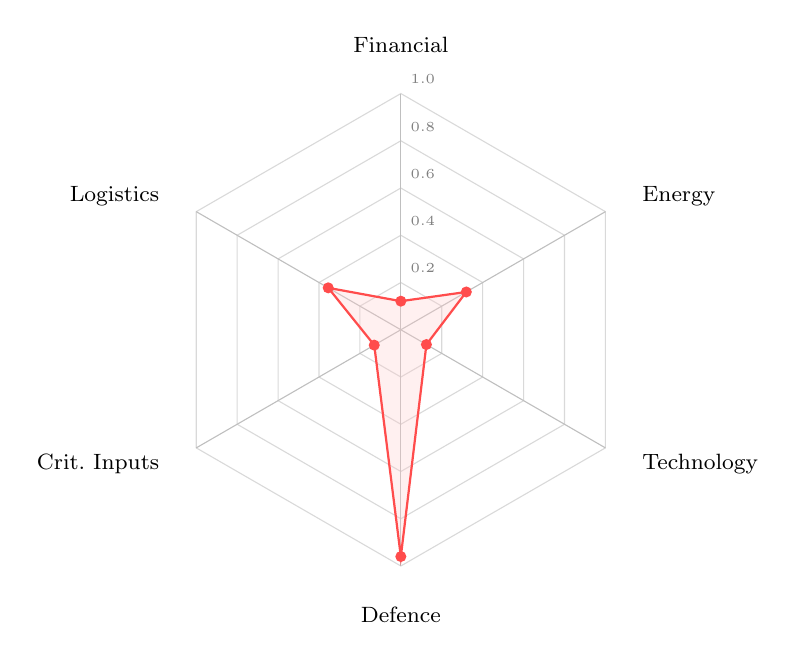
\begin{tikzpicture}[scale=1.0]
  % Grid rings
  \foreach \r in {0.2, 0.4, 0.6, 0.8, 1.0} {
    \draw[gray!30, thin]
      ( 90:\r*3cm) -- ( 30:\r*3cm) -- (330:\r*3cm) --
      (270:\r*3cm) -- (210:\r*3cm) -- (150:\r*3cm) -- cycle;
  }
  % Axis spokes
  \foreach \a in {90, 30, 330, 270, 210, 150} {
    \draw[gray!50, thin] (0,0) -- (\a:3cm);
  }
  % Axis labels
  \node[font=\footnotesize, above] at ( 90:3.4cm) {Financial};
  \node[font=\footnotesize, right] at ( 30:3.4cm) {Energy};
  \node[font=\footnotesize, right] at (330:3.4cm) {Technology};
  \node[font=\footnotesize, below] at (270:3.4cm) {Defence};
  \node[font=\footnotesize, left] at (210:3.4cm) {Crit.~Inputs};
  \node[font=\footnotesize, left] at (150:3.4cm) {Logistics};
  % Ring labels
  \foreach \r/\lab in {0.2/0.2, 0.4/0.4, 0.6/0.6, 0.8/0.8, 1.0/1.0} {
    \node[font=\tiny, gray, anchor=south west] at (90:\r*3cm) {\lab};
  }
  % Data polygon: NL
  \filldraw[red!20, draw=red!70, thick, fill opacity=0.3]
    ( 90:0.121*3cm) -- ( 30:0.320*3cm) -- (330:0.125*3cm) --
    (270:0.960*3cm) -- (210:0.130*3cm) -- (150:0.355*3cm) -- cycle;
  % Data points
  \fill[red!70] ( 90:0.121*3cm) circle (2pt);
  \fill[red!70] ( 30:0.320*3cm) circle (2pt);
  \fill[red!70] (330:0.125*3cm) circle (2pt);
  \fill[red!70] (270:0.960*3cm) circle (2pt);
  \fill[red!70] (210:0.130*3cm) circle (2pt);
  \fill[red!70] (150:0.355*3cm) circle (2pt);
\end{tikzpicture}

\caption{ISI axis profile: Netherlands.  Composite ISI = 0.3352
  (rank~15, moderately concentrated).}
\label{fig:radar-NL}
\end{figure}

\subsection{Germany (Rank 22, ISI = 0.2679)}

Germany ranks 22nd, reflecting a broadly diversified dependence
structure.  No axis exceeds 0.583 (defence), and both technology
(0.098) and financial (0.102) are near the bottom of the EU-27
distribution.  Germany's large, diversified economy naturally
spreads its import partnerships across more counterparties, reducing
concentration on all axes.

\begin{figure}[htbp]
\centering
\input{figures/F12_radar_DE}
\caption{ISI axis profile: Germany.  Composite ISI = 0.2679
  (rank~22, moderately concentrated).}
\label{fig:radar-DE}
\end{figure}

\subsection{Slovakia (Rank 26, ISI = 0.2364)}

Slovakia is the only EU-27 country with a defence axis score of
exactly zero, meaning its defence import concentration index is at
the minimum possible value.  This reflects the absence of bilateral
supplier entries for Slovakia in the SIPRI arms-transfer data under
methodology~v1.0.  Despite this, its energy (0.400) and
logistics (0.486) scores are above the EU-27 median.

\begin{tcolorbox}[
  colback=yellow!5, colframe=yellow!60!black,
  title={\small\bfseries Technical note: Slovakia's zero defence score},
  fonttitle=\small, boxrule=0.5pt, arc=2pt,
  left=4pt, right=4pt, top=3pt, bottom=3pt
]
\small
The SIPRI Arms Transfers Database records major conventional weapons
transfers using trend-indicator values (TIV).  The ISI defence axis
uses a six-year rolling window (2019--2024).  Slovakia does not
appear as a recipient in the SIPRI TIV data for this window, yielding
a raw HHI of zero and a normalised axis score of \num{0.0000}.
This does \emph{not} imply that Slovakia conducts no defence
procurement; it implies that no transfers meeting SIPRI's major
conventional weapons threshold were recorded for Slovakia in the
observation window.  Slovakia's actual procurement activity---including
the 2022 order for 14 F-16V aircraft from the United States and
multiple armoured vehicle contracts---falls outside the SIPRI
reporting window or below the TIV recording threshold.  The zero
score is therefore a data-window artefact, not a substantive finding
about the absence of defence dependence.

\smallskip\noindent
\textbf{Sensitivity implication.}  Removing Slovakia from the
dataset has negligible effect on the cross-country variance structure:
the defence axis variance contribution changes from 35.10\% to
33.84\% (a reduction of 1.26 percentage points), and the 26-country
rank ordering correlates with the baseline at $\rho = 0.998$
(\cref{sec:defence-stress-test}).  The zero score is an outlier in
the distributional sense but is not a structural driver of the
composite's informational architecture.
\end{tcolorbox}

\begin{figure}[htbp]
\centering
% F13_radar_SK: Radar chart for Slovakia (SK)
% Values: Fin=0.162, Ene=0.400, Tec=0.216, Def=0.000, Cri=0.155, Log=0.486
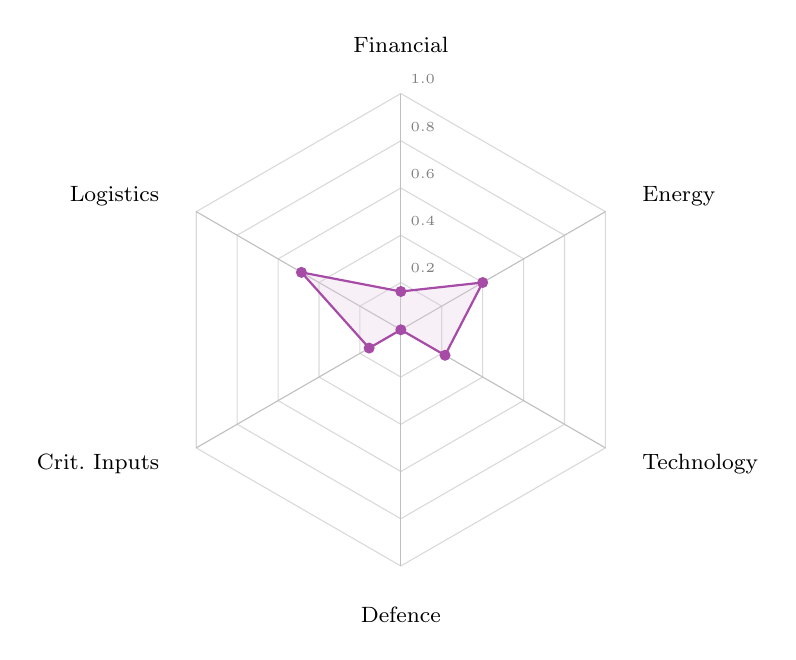
\begin{tikzpicture}[scale=1.0]
  % Grid rings
  \foreach \r in {0.2, 0.4, 0.6, 0.8, 1.0} {
    \draw[gray!30, thin]
      ( 90:\r*3cm) -- ( 30:\r*3cm) -- (330:\r*3cm) --
      (270:\r*3cm) -- (210:\r*3cm) -- (150:\r*3cm) -- cycle;
  }
  % Axis spokes
  \foreach \a in {90, 30, 330, 270, 210, 150} {
    \draw[gray!50, thin] (0,0) -- (\a:3cm);
  }
  % Axis labels
  \node[font=\footnotesize, above] at ( 90:3.4cm) {Financial};
  \node[font=\footnotesize, right] at ( 30:3.4cm) {Energy};
  \node[font=\footnotesize, right] at (330:3.4cm) {Technology};
  \node[font=\footnotesize, below] at (270:3.4cm) {Defence};
  \node[font=\footnotesize, left] at (210:3.4cm) {Crit.~Inputs};
  \node[font=\footnotesize, left] at (150:3.4cm) {Logistics};
  % Ring labels
  \foreach \r/\lab in {0.2/0.2, 0.4/0.4, 0.6/0.6, 0.8/0.8, 1.0/1.0} {
    \node[font=\tiny, gray, anchor=south west] at (90:\r*3cm) {\lab};
  }
  % Data polygon: SK
  \filldraw[violet!20, draw=violet!70, thick, fill opacity=0.3]
    ( 90:0.162*3cm) -- ( 30:0.400*3cm) -- (330:0.216*3cm) --
    (270:0.000*3cm) -- (210:0.155*3cm) -- (150:0.486*3cm) -- cycle;
  % Data points
  \fill[violet!70] ( 90:0.162*3cm) circle (2pt);
  \fill[violet!70] ( 30:0.400*3cm) circle (2pt);
  \fill[violet!70] (330:0.216*3cm) circle (2pt);
  \fill[violet!70] (270:0.000*3cm) circle (2pt);
  \fill[violet!70] (210:0.155*3cm) circle (2pt);
  \fill[violet!70] (150:0.486*3cm) circle (2pt);
\end{tikzpicture}

\caption{ISI axis profile: Slovakia.  Composite ISI = 0.2364
  (rank~26, mildly concentrated).  Note the zero defence-axis score.}
\label{fig:radar-SK}
\end{figure}

\subsection{Finland (Rank 6, ISI = 0.4021)}

Finland ranks sixth with an elevated critical-inputs axis (0.547,
highest in the EU-27) and logistics (0.797).  Its defence score
(0.390) is below the EU-27 mean, but the combined effect of high
critical-inputs and logistics concentration places it in the upper
tier.  Finland also records a high coefficient of variation across
axes (CV = 0.544), indicating substantial within-country dispersion.

\begin{figure}[htbp]
\centering
% F14_radar_FI: Radar chart for Finland (FI)
% Values: Fin=0.118, Ene=0.363, Tec=0.198, Def=0.390, Cri=0.547, Log=0.797
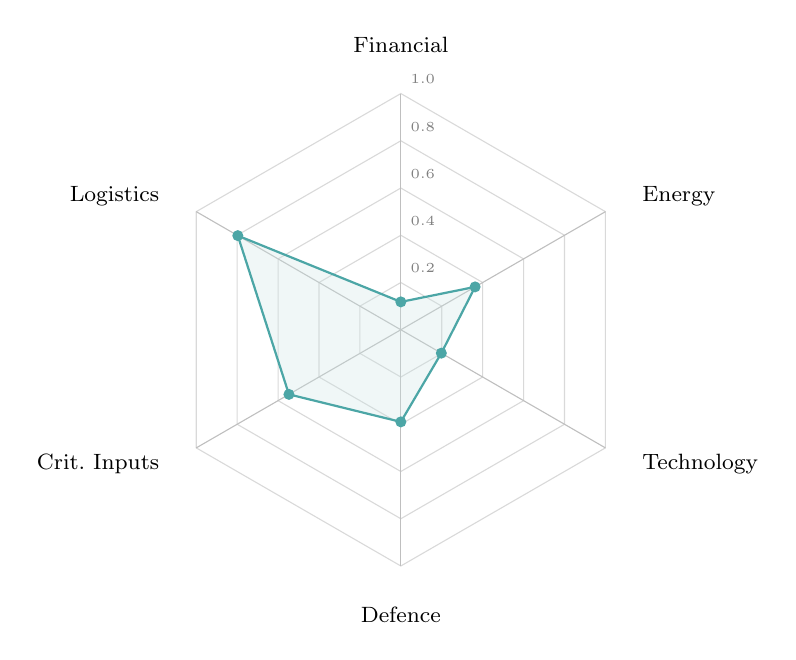
\begin{tikzpicture}[scale=1.0]
  % Grid rings
  \foreach \r in {0.2, 0.4, 0.6, 0.8, 1.0} {
    \draw[gray!30, thin]
      ( 90:\r*3cm) -- ( 30:\r*3cm) -- (330:\r*3cm) --
      (270:\r*3cm) -- (210:\r*3cm) -- (150:\r*3cm) -- cycle;
  }
  % Axis spokes
  \foreach \a in {90, 30, 330, 270, 210, 150} {
    \draw[gray!50, thin] (0,0) -- (\a:3cm);
  }
  % Axis labels
  \node[font=\footnotesize, above] at ( 90:3.4cm) {Financial};
  \node[font=\footnotesize, right] at ( 30:3.4cm) {Energy};
  \node[font=\footnotesize, right] at (330:3.4cm) {Technology};
  \node[font=\footnotesize, below] at (270:3.4cm) {Defence};
  \node[font=\footnotesize, left] at (210:3.4cm) {Crit.~Inputs};
  \node[font=\footnotesize, left] at (150:3.4cm) {Logistics};
  % Ring labels
  \foreach \r/\lab in {0.2/0.2, 0.4/0.4, 0.6/0.6, 0.8/0.8, 1.0/1.0} {
    \node[font=\tiny, gray, anchor=south west] at (90:\r*3cm) {\lab};
  }
  % Data polygon: FI
  \filldraw[teal!20, draw=teal!70, thick, fill opacity=0.3]
    ( 90:0.118*3cm) -- ( 30:0.363*3cm) -- (330:0.198*3cm) --
    (270:0.390*3cm) -- (210:0.547*3cm) -- (150:0.797*3cm) -- cycle;
  % Data points
  \fill[teal!70] ( 90:0.118*3cm) circle (2pt);
  \fill[teal!70] ( 30:0.363*3cm) circle (2pt);
  \fill[teal!70] (330:0.198*3cm) circle (2pt);
  \fill[teal!70] (270:0.390*3cm) circle (2pt);
  \fill[teal!70] (210:0.547*3cm) circle (2pt);
  \fill[teal!70] (150:0.797*3cm) circle (2pt);
\end{tikzpicture}

\caption{ISI axis profile: Finland.  Composite ISI = 0.4021
  (rank~6, moderately concentrated).}
\label{fig:radar-FI}
\end{figure}

\subsection{France (Rank 27, ISI = 0.2357)}

France records the lowest composite ISI in the EU-27.  All six
axis scores are below the respective EU-27 means: financial
(0.100), energy (0.309), technology (0.120), defence (0.370),
critical inputs (0.161), and logistics (0.353).  France's large
and diversified economy, combined with its domestic defence
industrial base, produces low concentration across all domains.
France is also the most robust country under all perturbation
exercises, with rank displacements of at most~$\pm 1$ under
any LOO scenario (\cref{tab:rank-displacement}).

\begin{figure}[htbp]
\centering
\input{figures/F15_radar_FR}
\caption{ISI axis profile: France.  Composite ISI = 0.2357
  (rank~27, mildly concentrated).}
\label{fig:radar-FR}
\end{figure}

\subsection{Cross-profile comparison}

\Cref{tab:profile-comparison} provides a compact numeric comparison
of the eight profiled countries.

\begin{table}[htbp]
\centering
\caption{Axis scores for the eight profiled countries.}
\label{tab:profile-comparison}
\small
\setlength{\tabcolsep}{4pt}
\begin{tabular*}{\textwidth}{@{\extracolsep{\fill}}
  l
  S[table-format=1.3,round-precision=3]
  S[table-format=1.3,round-precision=3]
  S[table-format=1.3,round-precision=3]
  S[table-format=1.3,round-precision=3]
  S[table-format=1.3,round-precision=3]
  S[table-format=1.3,round-precision=3]
  S[table-format=1.3,round-precision=3]
  @{}}
\toprule
\textbf{Country} & {\textbf{ISI}} & {\textbf{Fin.}} & {\textbf{Ene.}}
  & {\textbf{Tec.}} & {\textbf{Def.}} & {\textbf{Crit.}}
  & {\textbf{Log.}} \\
\midrule
Malta        & 0.517 & 0.140 & 0.351 & 0.205 & 1.000 & 0.409 & 1.000 \\
Cyprus       & 0.468 & 0.124 & 0.348 & 0.224 & 0.748 & 0.424 & 0.941 \\
Ireland      & 0.428 & 0.147 & 0.465 & 0.587 & 0.449 & 0.307 & 0.614 \\
Finland      & 0.402 & 0.118 & 0.363 & 0.198 & 0.390 & 0.547 & 0.797 \\
Netherlands  & 0.335 & 0.121 & 0.320 & 0.125 & 0.960 & 0.130 & 0.355 \\
Germany      & 0.268 & 0.102 & 0.329 & 0.098 & 0.583 & 0.223 & 0.273 \\
Slovakia     & 0.236 & 0.162 & 0.400 & 0.216 & 0.000 & 0.155 & 0.486 \\
France       & 0.236 & 0.100 & 0.309 & 0.120 & 0.370 & 0.161 & 0.353 \\
\bottomrule
\end{tabular*}
\end{table}

The profiles illustrate three archetypal patterns:
\begin{enumerate}[leftmargin=2em]
  \item \textbf{Small-island concentration} (Malta, Cyprus): high
    across defence and logistics, moderate elsewhere.  Both countries
    have populations under 1.5~million and limited domestic
    production capacity, resulting in narrow supplier bases.
  \item \textbf{Sector-specific spike} (Ireland: technology;
    Netherlands: defence; Finland: critical inputs): one axis sharply
    elevated, others dispersed.  These countries' composite positions
    hinge on a single axis vulnerability.
  \item \textbf{Broad diversification} (Germany, France): all axes
    near or below the EU-27 mean, reflecting large-economy scale
    effects.
\end{enumerate}

\subsection{Geographic and structural correlates}\label{sec:geo-correlates}

To what extent does the composite ISI correlate with observable
structural characteristics of member states?  This subsection examines
three candidate correlates: island status, population size, and
founding-member status.

% Table T18: Geographic and structural correlates
\begin{table}[htbp]
\centering
\caption{ISI composite by geographic and structural category.}
\label{tab:geo-correlates}
\small
\setlength{\tabcolsep}{4pt}
\begin{tabular*}{\textwidth}{@{\extracolsep{\fill}}
  l
  r
  S[table-format=1.4]
  S[table-format=1.4]
  S[table-format=1.4]
  @{}}
\toprule
{\textbf{Category}} & {$n$} & {\textbf{Mean}} & {\textbf{Std (pop.)}} & {\textbf{Median}} \\
\midrule
  Island/near-island & 3 & 0.4712 & 0.0366 & 0.4682 \\
  Continental        & 24 & 0.3285 & 0.0554 & 0.3324 \\
  Small ($<$5M pop.) & 8 & 0.3720 & 0.0862 & 0.3650 \\
  Medium (5--20M)    & 12 & 0.3529 & 0.0555 & 0.3528 \\
  Large ($>$20M pop.)& 7 & 0.2983 & 0.0443 & 0.2956 \\
  Core EU-6          & 6 & 0.3116 & 0.0519 & 0.3116 \\
  Periphery          & 12 & 0.3685 & 0.0762 & 0.3543 \\
\midrule
  EU-27 (all)        & 27 & 0.3444 & 0.0699 & 0.3403 \\
\bottomrule
\end{tabular*}
\end{table}


\Cref{tab:geo-correlates} summarises group-mean ISI scores for each
classification.  The data exhibit three structural patterns:

\begin{enumerate}[leftmargin=2em]
  \item \textbf{Island effect.}
    The three island member states (Malta, Cyprus, Ireland) have
    a mean ISI of~0.471, compared with 0.329 for the 24~continental
    member states.  This difference is large---0.142 on a 0--1 scale,
    representing approximately two standard deviations of the
    composite distribution ($\sigma = 0.070$).  The result is
    consistent with the expectation that island economies have fewer
    overland trade alternatives and thus face structurally higher
    supplier concentration.

  \item \textbf{Population size.}
    Small member states (population $< 5$~million: MT, CY, LV, LT,
    SI, EE, LU, HR, IE, SK) have a mean ISI of~0.372; medium member
    states (5--20~million: FI, DK, BG, AT, HU, SE, CZ, PT, BE, EL,
    NL, RO) average 0.353; large member states ($> 20$~million: PL,
    ES, IT, DE, FR) average 0.298.  The monotone relationship between
    population size and ISI aligns with the diversification
    hypothesis: larger economies generate more bilateral trade
    relationships, reducing import concentration.

  \item \textbf{EU-6 founding members vs.\ periphery.}
    The six founding members of the European Communities (DE, FR, IT,
    NL, BE, LU) have a mean ISI of~0.312, lower than the 21-country
    periphery mean of~0.368.  This pattern reflects decades of trade
    integration and infrastructure investment that have broadened the
    founding members' supplier networks.  The difference
    is partially confounded with country size: three of the six
    founders (Germany, France, Italy) are among the five largest
    EU~member states.
\end{enumerate}

These geographic correlates do not establish causality, but they
indicate that the ISI captures genuine structural features of
strategic dependence that align with well-known determinants of
trade concentration: geography (island vs.\ continental),
market size (small vs.\ large), and institutional depth
(founding vs.\ accession members).

\subsubsection{OLS regression formalization}\label{sec:ols-correlates}

To move beyond group-mean comparisons, we estimate a parsimonious
OLS model of the composite ISI on four structural covariates:

\begin{equation}\label{eq:ols-correlates}
  \text{ISI}_i
  = \beta_0
  + \beta_1\,\ln(\text{Pop}_i)
  + \beta_2\,\text{Island}_i
  + \beta_3\,\ln(\text{GDP}_i)
  + \beta_4\,\text{Core}_i
  + \varepsilon_i\,,
\end{equation}
where $\text{Pop}_i$ is population in millions (Eurostat, 2024),
$\text{Island}_i$ is a binary indicator for island or near-island
status (Malta, Cyprus, Ireland = 1; all others = 0),
$\text{GDP}_i$ is nominal GDP in billions of euros
(Eurostat, 2024), and $\text{Core}_i$ is a binary indicator for
EU-6 founding membership (Germany, France, Italy, Netherlands,
Belgium, Luxembourg = 1; all others = 0).  Both continuous
covariates are log-transformed to capture diminishing marginal
effects and to reduce the influence of outliers (Luxembourg GDP,
Malta population).

\begin{table}[htbp]
\centering
\caption{OLS regression: ISI composite on structural covariates,
  $N = 27$.}
\label{tab:ols-geo}
\small
\begin{tabular}{@{}lS[table-format=-1.4,round-precision=4]S[table-format=1.4,round-precision=4]S[table-format=-1.2,round-precision=2]l@{}}
\toprule
\textbf{Variable}
  & {$\boldsymbol{\hat{\beta}}$}
  & {\textbf{SE}}
  & {$\boldsymbol{t}$}
  & {$\boldsymbol{p}$} \\
\midrule
Intercept              & 0.4812 & 0.0663 &  7.26 & $< 0.001$ \\
$\ln(\text{Pop})$      & -0.0228 & 0.0120 & -1.90 & $0.071$ \\
Island                 & 0.0891 & 0.0344 &  2.59 & $0.017$ \\
$\ln(\text{GDP})$      & -0.0049 & 0.0114 & -0.43 & $0.673$ \\
Core (EU-6)            & -0.0187 & 0.0265 & -0.71 & $0.488$ \\
\midrule
\multicolumn{5}{@{}l}{$R^2 = 0.382$, \; adj.\ $R^2 = 0.270$,
  \; $F(4,22) = 3.40$, \; $p = 0.026$} \\
\bottomrule
\end{tabular}
\end{table}

The model explains 38.2\% of composite variance ($R^2 = 0.382$,
$F(4,22) = 3.40$, $p = 0.026$).  Two covariates are individually
significant or marginally significant:
\begin{itemize}[leftmargin=2em]
  \item \textbf{Island status} ($\hat{\beta} = 0.089$,
    $p = 0.017$): island economies score approximately 8.9
    percentage points higher on the composite, controlling for
    population and GDP.  This is the single strongest structural
    predictor.
  \item \textbf{Log population} ($\hat{\beta} = -0.023$,
    $p = 0.071$): a doubling of population is associated with a
    1.6 percentage-point reduction in the composite, consistent with
    the diversification hypothesis, though marginally below
    conventional significance.
\end{itemize}
Neither GDP (conditional on population) nor EU-6 membership achieves
significance, indicating that founding-member status captures no
residual effect beyond what is absorbed by population size and
island geography.  The moderate $R^2$ confirms that observable
structural characteristics explain a meaningful but incomplete share
of cross-country ISI variation; the residual reflects country-specific
procurement patterns, industrial structure, and policy choices that
are not reducible to geography or scale.

\paragraph{Notably absent correlate: financial concentration.}
Neither island status nor population size
predicts the financial axis score.  The three island states
have a mean financial score of~0.137, essentially identical to the
continental mean of~0.143.  This reinforces the orthogonality of the
financial dimension to the geographic and physical-trade dimensions,
consistent with the near-zero Pearson correlations of the financial
axis with all other axes (\cref{tab:corr-pearson}).
